\documentclass[colorlinks]{thesis-kando}
\usepackage[T1]{fontenc}
\PassOptionsToPackage{defaults=hu-min}{magyar.ldf}
\usepackage[magyar]{babel}
\usepackage{graphicx,amsmath,amssymb,amsthm,hulipsum,bussproofs}
\usepackage{listings,xcolor,rotating,booktabs,fancyvrb}
\usepackage{float}
\footnotestyle{rule=fourth}
\DeclareMathOperator{\tg}{tg}
\newtheorem{tetel}{Tétel}[chapter]
\newtheorem{lemma}[tetel]{Lemma}
\theoremstyle{definition}
\newtheorem{definicio}[tetel]{Definíció}
\newtheorem{feladat}[tetel]{Feladat}
\theoremstyle{remark}
\newtheorem{megjegyzes}[tetel]{Megjegyzés}
\newtheorem*{megoldas}{Megoldás}
\usepackage[normalem]{ulem}
\usepackage[linguistics]{forest}
\useunder{\uline}{\ul}{}
\usepackage{stackengine,scalerel}
\def\tang{\ThisStyle{\abovebaseline[0pt]{\scalebox{-1}{$\SavedStyle\perp$}}}}

% Define JavaScript language for listings
\lstdefinelanguage{JavaScript}{
	keywords={break, case, catch, continue, debugger, default, delete,
		do, else, finally, for, function, if, in, instanceof, new, return,
		switch, this, throw, try, typeof, var, void, while, with, let, const,
		export, import, await, async},
	ndkeywords={class, export, boolean, throw, implements, import, this, new},
	sensitive=true,
	comment=[l]{//},
	morecomment=[s]{/*}{*/},
	morestring=[b]',
	morestring=[b]",
	alsoletter={-},
	alsodigit={:},
	morekeywords=[2]{=>, yield, async, await, constructor},
	keywordstyle=\color{blue}\bfseries,
	ndkeywordstyle=\color{green}\bfseries,
	identifierstyle=\color{black},
	commentstyle=\color{gray}\ttfamily,
	stringstyle=\color{red}\ttfamily,
}

% Customize listings appearance
\lstset{
	language=JavaScript,
	extendedchars=true,
	inputencoding=utf8,
	basicstyle=\ttfamily\small,
	numbers=left,
	numberstyle=\tiny\color{gray},
	stepnumber=1,
	numbersep=10pt,
	showstringspaces=false,
	breaklines=true,
	frame=single,
	captionpos=b,
	escapeinside={\%*}{*)},
}

% Fordított 'T' szimbólum definiálása
\def\tang{\ThisStyle{\abovebaseline[0pt]{\scalebox{-1}{$\SavedStyle\perp$}}}}


\begin{document}

\title{Eseményrendező\\[1em]
	\begin{center}
		
\includegraphics[width=0.4\textwidth]{logo.jpg}
\end{center}}
\author{Pusztai Gábor\\ Iváncsik Ábrahám\\és Fehér Dominik\\Szoftverfejlesztő és -tesztelő szak}
\supervisor{Kerényi Róbert Nándor\\oktató}
\city{Miskolc}
\date{2025}
\maketitle

\tableofcontents

\chapter*{Bevezetés}
\addcontentsline{toc}{chapter}{Bevezetés}

A digitális világ folyamatos fejlődése során egyre fontosabbá vált a közösségek szerveződése és a személyes találkozások megkönnyítése, akár egy adott esemény keretében. Ezért döntöttünk úgy, hogy olyan rendszert tervezünk, amely egyszerűvé és átláthatóvá teszi az események létrehozását, valamint a részvételi visszajelzések kezelését.

 Az eseményszervezés kihívásai közé tartozik, hogy könnyen elérhető legyen a helyszín, minden résztvevő időben értesüljön a fontos részletekről, és a visszajelzések megfelelően legyenek kezelve. Az online platformok lehetővé teszik, hogy ezeket a problémákat egyetlen rendszerben oldjuk meg. Ez a projekt olyan funkciókat tartalmaz, mint a felhasználók regisztrációja és események létrehozása, amelyek egyaránt célozzák a személyes és professzionális eseményeket, például koncerteket, workshopokat, vagy előadásokat. Az egyszerűség érdekében a felhasználók könnyen bejelentkezhetnek, eseményeket hozhatnak létre, valamint interaktív módon visszajelzést adhatnak részvételükről.
 
  Az alkalmazás további előnyei közé tartozik a geolokációs integráció, amely lehetővé teszi, hogy a felhasználók pontosan meghatározzák az események helyszínét egy térképen keresztül. Ez a megoldás nemcsak a regisztrált, hanem a nem regisztrált felhasználók számára is biztosítja az eseményekre történő meghívás és részvétel lehetőségét, így szélesebb közönséget elérve. A projekt célja tehát egy olyan átfogó rendszer kialakítása, amely megkönnyíti az eseményszervezést és a résztvevők közti kommunikációt, egyúttal modern, interaktív és felhasználóbarát megoldásokat kínál.


\chapter{Technológiai háttér}

\section{Relációs Adatbáziskezelő Rendszerek}

A relációs adatbáziskezelő rendszerek (RDBMS) olyan szoftverek, amelyek az adatokat táblázatos formában tárolják, lehetővé téve az adatok közötti komplex kapcsolatok egyszerű kezelését. A relációs modell, amely a matematikai relációkon alapul, biztosítja, hogy az adatok logikusan és strukturáltan legyenek rendezve, ezáltal elősegítve az adatok hatékony keresését, lekérdezését és manipulálását.
\cite{relacio1}
Az RDBMS-ek legfontosabb jellemzője, hogy az adatok közötti kapcsolatokra fókuszálnak. Minden adatbázis egy vagy több táblából áll, ahol a táblák sorokból (rekordok) és oszlopokból (attribútumok) épülnek fel. A primér kulcs (egyedi azonosító) garantálja, hogy minden rekord egyedi legyen, míg az idegen kulcsok lehetővé teszik a táblák közötti kapcsolatok definiálását. Ezen kapcsolatok révén az RDBMS-ek lehetővé teszik az adatok integritásának fenntartását és a redundancia minimalizálását.

Az RDBMS-ek legfontosabb jellemzői közé tartozik a tranzakciókezelés, amely biztosítja az adatok konzisztenciáját. A tranzakciók atomitása, konzisztenciája, izolációja és tartóssága (ACID elvek) biztosítják, hogy egy műveletsorozat vagy teljes mértékben végrehajtódik, vagy egyáltalán nem, ezzel megelőzve az adatvesztést és a sérüléseket.

A legnépszerűbb relációs adatbáziskezelő rendszerek közé tartozik az Oracle, a Microsoft SQL Server, a PostgreSQL és a MySQL. Ezek a rendszerek széles körben használatosak különböző iparágakban, például a pénzügyi szolgáltatásokban, a kereskedelemben, az egészségügyben és a telekommunikációban. Az RDBMS-ek lehetővé teszik az adatok könnyű keresését és feldolgozását, így alapvető fontosságúak az üzleti intelligencia és az adatelemzés területén.

MySQL/MariaDB és PHPMyAdmin
A MySQL és a MariaDB a legelterjedtebb nyílt forráskódú relációs adatbáziskezelő rendszerek közé tartoznak. A MySQL, amelyet 1995-ben alapítottak, gyorsan népszerűvé vált a webes alkalmazások körében. 2010-ben, amikor a Sun Microsystems-t az Oracle Corporation megvásárolta, felmerültek aggályok a MySQL jövőjével kapcsolatban, így a MariaDB fejlesztése indult el, amely célja a MySQL funkcióinak és teljesítményének megőrzése és továbbfejlesztése.

A MySQL és a MariaDB közötti fő különbség az, hogy a MariaDB közösségi orientált, és folyamatosan új funkciókat és teljesítményjavításokat kínál. Mindkét rendszer nagy népszerűségnek örvend, mivel könnyen telepíthető, rugalmas, és nagy teljesítményt nyújt.

A MySQL és a MariaDB számos jellemzőt kínál, például:

1.Teljesítmény: Képesek nagy mennyiségű adat kezelésére és gyors lekérdezések végrehajtására.
2.Skálázhatóság: Könnyen bővíthetők, ami lehetővé teszi a nagy rendszerek kialakítását.
3.Biztonság: Támogatják a felhasználói jogosultságok és szerepkörök kezelését, így biztosítva, hogy csak a megfelelő felhasználók férhessenek hozzá az adatokhoz.
4.Tranzakciókezelés: Az ACID elveknek köszönhetően biztosítják az adatok integritását.

A PHPMyAdmin egy rendkívül népszerű webalapú alkalmazás, amely a MySQL és a MariaDB adatbázisok kezelésére szolgál. Az alkalmazás célja, hogy megkönnyítse a felhasználók számára az adatbázisokkal végzett műveletek elvégzését, anélkül hogy mélyebb technikai ismeretekre lenne szükség. Az intuitív felhasználói felület lehetővé teszi az adatok egyszerű kezelését, beleértve a táblák létrehozását, módosítását, törlését és lekérdezését.

A PHPMyAdmin főbb jellemzői a következők:

1.Grafikus felhasználói felület: Könnyen navigálható, lehetővé téve a felhasználók számára, hogy intuitív módon végezzenek műveleteket.
2.SQL lekérdezések végrehajtása: A felhasználók közvetlenül írhatnak és futtathatnak SQL lekérdezéseket, és megtekinthetik az eredményeket.
3.Adatbázisok importálása és exportálása: A PHPMyAdmin támogatja a különböző formátumokban történő adatimportálást és -exportálást, ami megkönnyíti az adatok mozgatását.
4.Felhasználói jogosultságok kezelése: A rendszergazdák képesek beállítani, hogy ki férhet hozzá az egyes adatbázisokhoz, ezzel biztosítva a biztonságot.
5.Adatok vizualizációja: A PHPMyAdmin grafikus ábrázolásokat kínál, amelyek segítségével a felhasználók könnyen megérthetik az adatok közötti kapcsolatokat.

A MySQL/MariaDB és a PHPMyAdmin kombinációja lehetővé teszi a fejlesztők és az adatkezelők számára, hogy hatékonyan kezeljék az adatbázisokat, és gyorsan reagáljanak az üzleti igényekre. A nyílt forráskódú természetük, a közösségi támogatás és a folyamatos fejlesztések miatt a MySQL és a MariaDB kiváló választás a modern adatbázis-kezelési igényekhez. Az ilyen rendszerek használata nemcsak a hatékonyságot növeli, hanem lehetővé teszi a felhasználók számára, hogy a legfrissebb technológiákat kihasználva fejlesszék alkalmazásaikat. Ezért döntötünk úgy , hogy ezeket használjuk a programunkhoz.

\section{.NET Web API}

A .NET Web API a Microsoft által fejlesztett keretrendszer, mely lehetővé teszi HTTP-alapú szolgáltatások létrehozását RESTful elvek mentén. Az alkalmazások fejlesztéséhez az ASP.NET Core Web API-t használják, amely a .NET Core platform része. Ez a technológia skálázható, jól tesztelhető és platformfüggetlen megoldást kínál API-k létrehozására.
\cite{net1}

Főbb jellemzői:

Egyszerűség: Kódolás közben kevés boilerplate kódra van szükség, így a fejlesztők gyorsan hozhatnak létre API-kat.

Integráció: Kiválóan integrálható különböző .NET alapú alkalmazásokkal és más platformokkal is.

Skálázhatóság: Alkalmas nagy volumenű, elosztott rendszerek kiszolgálására.

Biztonság: Erős támogatást nyújt különböző hitelesítési és jogosultsági rendszerekhez.

Az ASP.NET Core Web API lehetővé teszi a fejlesztők számára, hogy gyorsan és hatékonyan készítsenek webszolgáltatásokat, melyek könnyen karbantarthatók és bővíthetők. Az ilyen API-k segítségével különböző kliensek, például webes és mobil alkalmazások könnyedén hozzáférhetnek az adatokhoz és funkciókhoz.

\section{A React Programozás Alapjai és Fejlettebb Fogalmai}

Bevezetés
A React egy JavaScript könyvtár, amelyet a Facebook fejlesztett ki 2013-ban. A React célja, hogy segítse a fejlesztőket dinamikus, interaktív felhasználói felületek (UI) építésében, különösen a webalkalmazások esetében. A könyvtár elterjedésével és folyamatos fejlődésével ma már szinte az iparági szabvánnyá vált a modern webalkalmazások fejlesztésében. A React alapelve az, hogy a felhasználói felületet komponens-alapú módon kell felépíteni, ahol minden komponens önálló, újrahasznosítható és kezelhető.
\cite{react1}

A React egyik legfontosabb előnye a virtuális DOM használata, amely lehetővé teszi az alkalmazás gyors és hatékony frissítését anélkül, hogy a teljes dokumentumot újra renderelni kellene. A React fejlesztése gyors, a kód karbantartása könnyű, és lehetővé teszi a dinamikus, interaktív alkalmazások gyors prototípusát.

1. React Alapfogalmak
1.1 Komponens-alapú fejlesztés
A React alkalmazások a komponensek köré épülnek. A komponens egy önálló kódrészlet, amely egy adott funkciót vagy vizuális elemet képvisel a felhasználói felületen. Mivel a komponensek kis egységek, újrahasznosíthatók, és könnyen karbantarthatók, a kód tiszta és moduláris marad.

A komponensek lehetnek:

Funkcionális komponensek: Ezek a legegyszerűbb típusú komponensek, amelyek JavaScript függvényekből állnak. A React 16.8 verziójától kezdve funkcionális komponensek is rendelkezhetnek hookokkal, amelyek lehetővé teszik számukra az állapot kezelését és egyéb életciklus-műveletek végrehajtását.
Osztály-alapú komponensek: A React korábbi verzióiban ezek a komponensek voltak a standardok, és lehetővé tették az állapotok kezelését, valamint a komponens életciklusának vezérlését.
1.2 JSX
A React egyik legfontosabb jellemzője a JSX (JavaScript XML) szintaxis, amely lehetővé teszi, hogy HTML-t írjunk közvetlenül a JavaScript kódba. Ez a szintaxis egyszerűsíti a komponensek felépítését, és tiszta, olvasható kódot eredményez.

Példa JSX-re:
\begin{lstlisting}[language=JavaScript]
const element = <h1>Hello, world!</h1>;
\end{lstlisting}
A JSX kódot a React a háttérben JavaScript objektumokká fordítja, amiket aztán a virtuális DOM-ban kezel.

1.3 Virtuális DOM
A React egy virtuális DOM-ot használ a weboldalak renderelésének optimalizálására. Amikor a komponens állapota vagy a props változik, a React először a virtuális DOM-ban végzi el az összes változást, majd összehasonlítja azt a valódi DOM-mal. Csak azokat az elemeket frissíti, amelyek ténylegesen változtak, ezáltal gyorsabbá és hatékonyabbá téve az alkalmazás működését.

2. Állapot és Props
2.1 Állapotkezelés (State)
A state a React-ben egy komponens saját adatainak tárolására szolgál. Az állapot lehetővé teszi, hogy a komponens dinamikusan reagáljon a felhasználói interakciókra, például gombnyomásra, adatbevitelre, vagy bármely más eseményre. Az állapot kezelése a useState hook segítségével történik funkcionális komponensek esetén.

Példa egy egyszerű számláló alkalmazásra, amely az állapot kezelését mutatja be:
\begin{lstlisting}[language=JavaScript]
import React, { useState } from 'react';

function Counter() {
	const [count, setCount] = useState(0);
	
	return (
	<div>
	<p>Count: {count}</p>
	<button onClick={() => setCount(count + 1)}>Increment</button>
	</div>
	);
}
	

\end{lstlisting}


Ebben a példában a count az állapot, és a setCount egy függvény, amellyel módosíthatjuk az állapotot. Minden alkalommal, amikor az állapot frissül, a React újra rendereli a komponenst.

2.2 Props
A props (properties) egy olyan mechanizmus, amely lehetővé teszi, hogy adatokat adjunk át egy komponensnek a szülőkomponensből. A props-okat nem lehet módosítani a gyermek komponensben, csak olvasni.

Példa a props használatára:
\begin{lstlisting}[language=JavaScript]
function Greeting(props) {
	return <h1>Hello, {props.name}!</h1>;
}

function App() {
	return <Greeting name="Alice" />;
}

	
\end{lstlisting}


Itt az App komponens átadja az Alice értéket a Greeting komponensnek a name prop-on keresztül. A props segítségével a komponens adatokat kap, amelyek befolyásolják a megjelenített tartalmat.

3. Hookok
A React 16.8-as verziójától kezdve a hookok jelentik a legmodernebb módot az állapot és életciklus-műveletek kezelésére funkcionális komponensekben. A hookok lehetővé teszik, hogy a komponensek állapotot kezeljenek és reagáljanak a különböző életciklus eseményekre anélkül, hogy osztályokat kellene használni.

A leggyakoribb hookok:

useState: Állapot kezelésére szolgál.
useEffect: Mellékhatások kezelésére használják, mint például API hívások vagy események kezelése.
useContext: A React kontextus API-ját használja, amely lehetővé teszi az adatok globális kezelését a komponensek között.
useReducer: Összetettebb állapotkezeléshez használható, különösen olyan esetekben, amikor az állapot több részletből áll és a frissítések komplexek.
Példa a useEffect hook használatára:
\begin{lstlisting}[language=JavaScript]
	import React, { useState, useEffect } from 'react';
	
	function Timer() {
	const [seconds, setSeconds] = useState(0);
		
	useEffect(() => {
	const interval = setInterval(() => {
	setSeconds(prev => prev + 1);
	}, 1000);
			
	return () => clearInterval(interval); 
	// Takaritas, amikor a komponens eltunik
	}, []);
		
	return <h1>{seconds} seconds</h1>;
	}
\end{lstlisting}




Itt a useEffect minden egyes másodpercben frissíti a másodpercek számát, és amikor a komponens eltűnik, törli az időzítőt.

4. React Router és Navigáció
A React Router egy olyan könyvtár, amely lehetővé teszi, hogy különböző URL-ekhez rendeljünk React komponenseket. Ezáltal egyoldalas alkalmazásokat (SPA) hozhatunk létre, ahol a navigáció nem okoz teljes oldalbetöltést, hanem csak az adott komponens frissül.

Példa a React Router alapvető használatára:

import { BrowserRouter as Router, Route, Switch } from 'react-router-dom';

\begin{lstlisting}[language=JavaScript]
function App() {
	return (
	<Router>
	<Switch>
	<Route path="/" exact>
	<Home />
	</Route>
	<Route path="/about">
	<About />
	</Route>
	</Switch>
	</Router>
	);
}
\end{lstlisting}


5. Teljes React Alkalmazás Példa
Most nézzünk egy egyszerű alkalmazást, amely egy számlálót és egy gombot tartalmaz. A React alkalmazás alapját képező komponensek és állapotkezelés látható:

\begin{lstlisting}[language=JavaScript]
import React, { useState } from 'react';

function App() {
	const [count, setCount] = useState(0);
	
	return (
	<div>
	<h1>React Counter</h1>
	<p>Count: {count}</p>
	<button onClick={() => setCount(count + 1)}>Increment</button>
	<button onClick={() => setCount(count - 1)}>Decrement</button>
	</div>
	);
}
\end{lstlisting}
export default App;
Ebben a példában a useState hook-ot használjuk a count változó és a hozzá tartozó frissítő függvény (setCount) kezelésére. Két gomb segítségével növelhetjük és csökkenthetjük a számlálót.

6. Összegzés
A React a modern webalkalmazások egyik legnépszerűbb könyvtára, amely a komponens-alapú fejlesztést és a virtuális DOM használatát helyezi előtérbe. Az alapoktól kezdve a fejlettebb témákig, mint a hookok és az állapotkezelés, a React segít a gyors és dinamikus alkalmazások létrehozásában. Az alkalmazások modularitása és újrahasznosíthatósága biztosítja a könnyű karbantartást és skálázhatóságot, miközben a teljesítmény is kiváló a virtuális DOM-nak köszönhetően. Ahogy az ökoszisztéma folyamatosan fejlődik, a React továbbra is alapvető eszköze marad a front-end fejlesztők számára.

\section {CRUD Műveletek} 
A .NET Web API-ban a CRUD (Create, Read, Update, Delete) műveletek azok az alapvető műveletek, amelyeket egy adatbázis-kezelő rendszerben kell implementálni az adatok manipulálására. A .NET Web API-ban minden CRUD művelethez egy HTTP metódust rendelünk:
\cite{cr1}

\par Create: Az új adat létrehozása (HTTP POST).
\par Read: Az adat lekérése (HTTP GET).
\par Update: A meglévő adat módosítása (HTTP PUT/PATCH).
\par Delete: Az adat törlése (HTTP DELETE).
Példa CRUD műveletek ASP.NET Core Web API-ban:
Tegyük fel, hogy van egy Product nevű entitásunk, és létre akarunk hozni egy API-t, amely képes a termékek CRUD műveleteit végrehajtani.

\begin{lstlisting}[language=JavaScript]
public class Product
{
	public int Id { get; set; }
	public string Name { get; set; }
	public decimal Price { get; set; }
}
[Route("api/[controller]")]
[ApiController]

public class ProductsController : ControllerBase
{
	private static List<Product> _products = new List<Product>();
	
	// CREATE
	[HttpPost]
	public ActionResult<Product> CreateProduct(Product product)
	{
		product.Id = _products.Count + 1; // Generáljunk egy ID-t
		_products.Add(product);
		return CreatedAtAction(nameof(GetProduct), new { id = product.Id }, product);
	}
	
	// READ (Get all products)
	[HttpGet]
	public ActionResult<IEnumerable<Product>> GetProducts()
	{
		return Ok(_products);
	}
	
	// READ (Get a single product)
	[HttpGet("{id}")]
	public ActionResult<Product> GetProduct(int id)
	{
		var product = _products.FirstOrDefault(p => p.Id == id);
		if (product == null)
		return NotFound();
		return Ok(product);
	}
	
	// UPDATE
	[HttpPut("{id}")]
	public IActionResult UpdateProduct(int id, Product updatedProduct)
	{
		var product = _products.FirstOrDefault(p => p.Id == id);
		if (product == null)
		return NotFound();
		
		product.Name = updatedProduct.Name;
		product.Price = updatedProduct.Price;
		return NoContent(); // Successful update (no content returned)
	}
	
	// DELETE
	[HttpDelete("{id}")]
	public IActionResult DeleteProduct(int id)
	{
		var product = _products.FirstOrDefault(p => p.Id == id);
		if (product == null)
		return NotFound();
		
		_products.Remove(product);
		return NoContent(); // Successful deletion (no content returned)
	}
}
\end{lstlisting}
Ebben a példában a ProductsController osztály kezeli a CRUD műveleteket egy statikus listán, amely itt csak demonstrációs célt szolgál. Egy valós alkalmazásban ezek az adatok adatbázisban tárolódnának, például az Entity Framework segítségével.

2. API Tesztelés Swagger és Postman segítségével
Miután a Web API-t implementáltuk, érdemes biztosítani, hogy az API végpontok megfelelően működnek. Erre szolgálnak a tesztelési eszközök, mint a Swagger és a Postman.
Swagger:
A Swagger (vagy más néven OpenAPI Specification) egy dokumentációs és tesztelési eszköz, amely lehetővé teszi a fejlesztők számára, hogy könnyedén dokumentálják és teszteljék a Web API-kat. Az ASP.NET Core projektek automatikusan generálhatnak Swagger dokumentációt az API végpontjairól.

Swagger Integrálása az ASP.NET Core Web API-ban
Swagger csomag hozzáadása:

Az ASP.NET Core alkalmazáshoz hozzá kell adni a Swashbuckle.AspNetCore csomagot, amely lehetővé teszi a Swagger használatát. A NuGet Package Manager segítségével telepíthetjük:

bash

dotnet add package Swashbuckle.AspNetCore
Swagger konfigurálása az Startup.cs fájlban:

A Swagger konfigurálását a Startup.cs fájlban végezzük el. A ConfigureServices metódusban regisztráljuk a Swagger szolgáltatásokat, míg a Configure metódusban beállítjuk a Swagger middleware-t.


\begin{lstlisting}[language=JavaScript]
public void ConfigureServices(IServiceCollection services)
{
	services.AddControllers();
	services.AddSwaggerGen(c =>
	{
		c.SwaggerDoc("v1", new OpenApiInfo { Title = "Product API", Version = "v1" });
	});
}

public void Configure(IApplicationBuilder app, IWebHostEnvironment env)
{
	if (env.IsDevelopment())
	{
		app.UseSwagger();
		app.UseSwaggerUI(c => c.SwaggerEndpoint("/swagger/v1/swagger.json", "Product API v1"));
	}
	
	app.UseRouting();
	app.UseEndpoints(endpoints =>
	{
		endpoints.MapControllers();
	});
}
\end{lstlisting}

Swagger UI használata:

Ha elindítjuk az alkalmazást, a Swagger automatikusan generálja a dokumentációt az API végpontokhoz. A Swagger UI elérhető lesz a következő URL-en: https://localhost:<port>/swagger. Itt tesztelhetjük az API végpontokat a böngészőn keresztül.

Postman:
A Postman egy másik népszerű eszköz, amely lehetővé teszi az API-k tesztelését. A Postman segítségével egyszerűen küldhetünk HTTP kéréseket (GET, POST, PUT, DELETE) a végpontokhoz, és ellenőrizhetjük a válaszokat.

Postman Tesztelés
API hívások létrehozása:

A Postman-ben új kérés létrehozásához válasszuk ki a megfelelő HTTP metódust (pl. POST, GET, PUT, DELETE) és írjuk be a kért URL-t (pl. http://localhost:5000/api/products).

Kérés testreszabása: ~
GET kérés esetén egyszerűen kattintsunk a "Send" gombra, hogy lekérjük az adatokat. POST kérés esetén a kérés testében (Body) átadhatjuk a létrehozandó objektumot JSON formátumban, például:

\hspace*{1cm}

\begin{lstlisting}[language=JavaScript]
{
	"name": "New Product",
	"price": 19.99
}
\end{lstlisting}
Válasz ellenőrzése:

A Postman a válaszokat különböző formátumokban (pl. JSON, XML) jeleníti meg, és automatikusan ellenőrzi az állapotkódokat (pl. 200 OK, 404 Not Found). Emellett aserciókat (ellenőrzéseket) is hozzáadhatunk, hogy automatikusan validáljuk a válaszokat, például:

Status code: 200 OK
Response body: Ellenőrizzük, hogy a válasz tartalmazza-e a megfelelő adatokat.
3. Tesztelési Legjobb Gyakorlatok
Automatikus tesztelés: A Swagger és a Postman mellett automatizált teszteket is írhatunk, például xUnit vagy NUnit tesztelési keretrendszerekkel.
Környezeti beállítások: Fontos, hogy a teszteléshez megfelelő környezetet állítsunk be. Használjunk például fejlesztői és teszt környezetet, ahol az API végpontok működését validálhatjuk.
Adatellenőrzés: Teszteljük le, hogy az API megfelelően kezeli-e a bemeneti adatokat, és hogy hibás bemenet esetén megfelelő hibát generál-e.
Összegzés
A CRUD műveletek implementálása és tesztelése egy .NET Web API-ban viszonylag egyszerűen elvégezhető az ASP.NET Core és a megfelelő tesztelési eszközök segítségével. A Swagger és a Postman két olyan eszköz, amelyek jelentősen megkönnyítik az API tesztelését és dokumentálását. A Swagger UI lehetővé teszi az API.

\section {Entity Framework (EF) - Adatbázis kezelés}
Az Entity Framework egy objektum-relációs leképezési (ORM) eszköz a .NET platform számára, amely lehetővé teszi, hogy az adatbázisokat objektumokként kezeljük. Az EF segítségével nem kell SQL lekérdezéseket manuálisan írni, mert az ORM automatikusan leképezi az adatbázist és az objektumokat egymásra. Az Entity Framework használatával könnyen végezhetünk CRUD műveleteket (Create, Read, Update, Delete) az adatbázisban.
\cite{en1}

Példa:

Adatmodell: A User entitás például egy táblát reprezentálhat az adatbázisban.

\begin{lstlisting}[language=JavaScript]
public class User
{
	public int Id { get; set; }
	public string Name { get; set; }
	public string Email { get; set; }
}
\end{lstlisting}
DbContext: Az Entity Framework által használt kontextusosztály.

\begin{lstlisting}[language=JavaScript]
public class ApplicationDbContext : DbContext
{
	public DbSet<User> Users { get; set; }
}
\end{lstlisting}
\section {Web API - Backend kommunikáció}
A Web API az a közvetítő réteg, amely lehetővé teszi a frontend és a backend közötti kommunikációt HTTP protokollon keresztül. A Web API-t a .NET Core vagy .NET 6/7/8 környezetben fejleszthetjük, és RESTful szabványokat követhetünk a különböző műveletek (GET, POST, PUT, DELETE) kezelésére.
\cite{we1}

API Controller példa:
\begin{lstlisting}[language=JavaScript]
[ApiController]
[Route("api/[controller]")]
public class UsersController : ControllerBase
{
	private readonly ApplicationDbContext _context;
	
	public UsersController(ApplicationDbContext context)
	{
		_context = context;
	}
	
	[HttpGet]
	public async Task<ActionResult<IEnumerable<User>>> GetUsers()
	{
		return await _context.Users.ToListAsync();
	}
	
	[HttpPost]
	public async Task<ActionResult<User>> PostUser(User user)
	{
		_context.Users.Add(user);
		await _context.SaveChangesAsync();
		return CreatedAtAction(nameof(GetUsers), new { id = user.Id }, user);
	}
}
\end{lstlisting}
\section {React - Frontend}
A React egy JavaScript könyvtár, amelyet a Facebook fejlesztett ki és az interaktív felhasználói felületek építésére szolgál. A React alkalmazásokat a komponensek és a "state"-ek kezelése alapján fejlesztjük, és könnyen összekapcsolhatjuk backend API-kkal.

A React használatával egyszerűen integrálhatunk HTTP kéréseket a backend API-hoz, például a fetch API vagy külső könyvtárak, mint az Axios segítségével.
Példa: API hívás egy React komponensből:
\begin{lstlisting}[language=JavaScript]
import React, { useEffect, useState } from 'react';
function App() {
	const [users, setUsers] = useState([]);
	
	useEffect(() => {
		fetch('https://localhost:5001/api/users')
		.then((response) => response.json())
		.then((data) => setUsers(data));
	}, []);
	
	return (
	<div>
	<h1>User List</h1>
	<ul>
	{users.map(user => (
		<li key={user.id}>{user.name}</li>
		))}
	</ul>
	</div>
	);
}
export default App;
\end{lstlisting}
\section {Integráció - React és Web API}
A frontend React alkalmazás és a backend Web API közötti kommunikációt RESTful API-val érhetjük el. Az API válaszként JSON formátumban küldi az adatokat, amelyeket a React komponensekben felhasználhatunk. A HTTP kérések (GET, POST, PUT, DELETE) segítségével CRUD műveleteket végezhetünk.

JSON válaszok: Az Entity Framework és a Web API együtt dolgozik, hogy az adatokat JSON formátumban küldje vissza a frontendnek.
Axios vagy fetch API: Az Axios könyvtárat használhatjuk, hogy HTTP kéréseket küldjünk az API-nak.
\par
5. Összefoglaló
Backend: Az Entity Framework és a Web API kombinálásával egy erős adatbázis-kezelési réteget hozhatunk létre, amely lehetővé teszi a dinamikus adatfeldolgozást és kommunikációt az adatbázissal.
Frontend: A React segítségével dinamikus és interaktív felhasználói felületet építhetünk, amely könnyedén összekapcsolható az API-val, hogy adatokat kérjünk és jelenítsünk meg.
Ez a kombináció a modern webfejlesztés alapja, és nagyban javítja a fejlesztési folyamatot, miközben biztosítja a skálázhatóságot és az egyszerű karbantartást.
\chapter{Program}

\section{Adatbázis}
Ez az SQL szkript három különböző táblát tartalmaz, amelyeket egy eseményrendező rendszerhez terveztünk. A három tábla az alábbiak szerint van kialakítva:

\subsection{Felhasználó}
Ez a tábla a felhasználók adatait tartalmazza, beleértve a felhasználó nevét, teljes nevét, email címét, jogosultságait, aktivitási státuszát, valamint a regisztráció időpontját és egyéb kapcsolódó adatokat. A tábla segítségével nyomon követhetjük a felhasználói fiókokat és jogosultságokat, biztosítva a megfelelő hozzáférést a rendszer különböző funkcióihoz.

\subsection{Esemény}
Az eseménytáblában különböző rendezvények információit tároljuk, beleértve az esemény nevét, helyszínét, dátumát, leírását és a kapcsolódó képet. Ez a tábla lehetővé teszi a különböző események könnyű kezelését és megjelenítését a rendszerben.

\subsection{Chat üzenetek}
Ez a tábla a felhasználók közötti üzenetváltásokat tárolja, amelyben szerepel az üzenet ID-ja, a felhasználó neve, az üzenet szövege és az üzenet küldésének időpontja. A tábla használata lehetővé teszi a chat üzenetek rögzítését és későbbi visszakeresését.

\noindent 
A rendszer ezen táblák segítségével hatékonyan képes kezelni a felhasználók közötti kommunikációt, az események szervezését és a felhasználói adatokat. Az adatbázis felépítése biztosítja a rugalmas és átlátható működést, lehetővé téve a könnyű adatkezelést és a jövőbeli bővítéseket.

 \section{Backend}
 
 A backend rendszer a .NET Core keretrendszerre épül, amely biztosítja a szükséges infrastruktúrát a webes API-k létrehozásához és az adatbázis-kezeléshez. Az alábbiakban részletesen bemutatjuk a backend komponenseit és működését.
 
 \subsection{Kontrollerek}
 
 A kontrollerek felelősek a HTTP kérések kezeléséért és a megfelelő válaszok visszaküldéséért. Az alkalmazás a következő fő kontrollereket tartalmazza:
 
 \subsubsection{EsemenyController}
 
 Az \texttt{EsemenyController} felelős az események kezeléséért:
 
 \begin{itemize}
 	\item \textbf{GET /api/Esemeny}: Összes esemény lekérdezése
 	\item \textbf{GET /api/Esemeny/\{id\}}: Egy adott esemény lekérdezése azonosító alapján
 	\item \textbf{POST /api/Esemeny}: Új esemény létrehozása
 	\item \textbf{PUT /api/Esemeny/\{id\}}: Meglévő esemény frissítése
 	\item \textbf{DELETE /api/Esemeny/\{id\}}: Esemény törlése
 \end{itemize}
 
 Az eseményekhez kapcsolódó műveletek jogosultságkezelést tartalmaznak, bizonyos műveletek csak bejelentkezett felhasználók vagy adminisztrátorok számára érhetők el.
 
 \subsubsection{FelhasznaloController}
 
 A \texttt{FelhasznaloController} a felhasználói fiókokkal kapcsolatos műveleteket kezeli:
 
 \begin{itemize}
 	\item \textbf{POST /api/Felhasznalo/register}: Felhasználói regisztráció
 	\item \textbf{POST /api/Felhasznalo/login}: Bejelentkezés
 	\item \textbf{POST /api/Felhasznalo/logout}: Kijelentkezés
 	\item \textbf{GET /api/Felhasznalo/profile}: Felhasználói profil lekérdezése
 	\item \textbf{PUT /api/Felhasznalo/profile}: Profil adatok frissítése
 	\item \textbf{POST /api/Felhasznalo/refresh-token}: Token frissítése
 	\item \textbf{POST /api/Felhasznalo/change-password}: Jelszó módosítása
 \end{itemize}
 
 A kontroller tartalmazza a szükséges biztonsági ellenőrzéseket, beleértve a jelszó validációt és a token kezelést.
 
 \subsubsection{ReszvetelController}
 
 A \texttt{ReszvetelController} az eseményeken való részvételt kezeli:
 
 \begin{itemize}
 	\item \textbf{POST /api/Reszvetel}: Részvétel regisztrálása egy eseményre
 	\item \textbf{GET /api/Reszvetel/user/\{userId\}}: Felhasználó részvételeinek lekérdezése
 	\item \textbf{GET /api/Reszvetel/event/\{eventId\}}: Eseményen résztvevők lekérdezése
 	\item \textbf{DELETE /api/Reszvetel/\{id\}}: Részvétel törlése
 \end{itemize}
 
 \subsection{Szolgáltatások (Services)}
 
 \subsubsection{TokenService}
 
 A \texttt{TokenService} felelős a JWT tokenek kezeléséért:
 
 \begin{itemize}
 	\item \textbf{GenerateAccessToken}: Hozzáférési token generálása
 	\item \textbf{GenerateRefreshToken}: Frissítési token generálása
 	\item \textbf{ValidateToken}: Token érvényességének ellenőrzése
 	\item \textbf{GetPrincipalFromExpiredToken}: Lejárt tokenből felhasználói adatok kinyerése
 \end{itemize}
 
 \subsubsection{EmailService}
 
 Az \texttt{EmailService} az e-mail küldési funkcionalitást biztosítja:
 
 \begin{itemize}
 	\item \textbf{SendRegistrationConfirmation}: Regisztrációs visszaigazolás küldése
 	\item \textbf{SendPasswordReset}: Jelszó-visszaállítási e-mail küldése
 	\item \textbf{SendEventNotification}: Esemény értesítések küldése
 \end{itemize}
 
 \subsection{Middleware-ek}
 
 \subsubsection{AuthenticationMiddleware}
 
 Az \texttt{AuthenticationMiddleware} minden kérés esetén ellenőrzi a felhasználó hitelesítését:
 
 \begin{itemize}
 	\item JWT token validálása
 	\item Felhasználói jogosultságok ellenőrzése
 	\item Munkamenet kezelése
 \end{itemize}
 
 \subsubsection{ExceptionHandlingMiddleware}
 
 Az \texttt{ExceptionHandlingMiddleware} a hibakezelésért felelős:
 
 \begin{itemize}
 	\item Kivételek elfogása és naplózása
 	\item Megfelelő HTTP státuszkódok visszaadása
 	\item Hibaüzenetek formázása a kliensek számára
 \end{itemize}
 
 \subsection{Adatbázis Műveletek}
 
 \subsubsection{Repository Pattern}
 
 Az alkalmazás a Repository mintát használja az adatbázis-műveletek absztrahálására:
 
 \begin{itemize}
 	\item \textbf{IEsemenyRepository}: Események CRUD műveletei
 	\item \textbf{IFelhasznaloRepository}: Felhasználók kezelése
 	\item \textbf{IReszvetelRepository}: Részvételek kezelése
 \end{itemize}
 
 \subsubsection{Entity Framework Core}
 
 Az adatbázis-műveletek Entity Framework Core segítségével történnek:
 
 \begin{itemize}
 	\item Code-First megközelítés
 	\item Migrációk kezelése
 	\item Kapcsolatok definiálása a modellek között
 \end{itemize}
 
 \subsection{API Biztonság}
 
 \subsubsection{CORS Konfiguráció}
 
 A Cross-Origin Resource Sharing (CORS) beállítások lehetővé teszik a frontend és backend közötti biztonságos kommunikációt:
 
 \begin{lstlisting}[language=csharp]
 	services.AddCors(options =>
 	{
 		options.AddPolicy("AllowSpecificOrigin",
 		builder => builder
 		.WithOrigins("http://localhost:3000")
 		.AllowAnyMethod()
 		.AllowAnyHeader()
 		.AllowCredentials());
 	});
 \end{lstlisting}
 
 \subsubsection{Rate Limiting}
 
 A túlzott API-hívások elleni védelem érdekében rate limiting van implementálva:
 
 \begin{itemize}
 	\item IP-alapú korlátozások
 	\item Időablak-alapú korlátozások
 	\item Különböző korlátozások különböző végpontokra
 \end{itemize}
 
 \subsection{Naplózás}
 
 A backend részletes naplózási rendszerrel rendelkezik:
 
 \begin{itemize}
 	\item \textbf{Serilog} integrációja
 	\item Strukturált naplózás
 	\item Különböző naplózási szintek (Debug, Information, Warning, Error)
 	\item Naplófájlok rotációja
 \end{itemize}
 
 \subsection{Teljesítmény Optimalizáció}
 
 \subsubsection{Gyorsítótárazás}
 
 Az alkalmazás memória-gyorsítótárat használ a gyakran lekérdezett adatok gyorsabb elérése érdekében:
 
 \begin{itemize}
 	\item Események listájának gyorsítótárazása
 	\item Felhasználói profilok gyorsítótárazása
 	\item Időalapú gyorsítótár-érvénytelenítés
 \end{itemize}
 
 \subsubsection{Aszinkron Műveletek}
 
 A backend aszinkron műveleteket használ a skálázhatóság és teljesítmény érdekében:
 
 \begin{itemize}
 	\item Aszinkron kontroller műveletek
 	\item Task-alapú adatbázis-műveletek
 	\item Nem blokkoló I/O műveletek
 \end{itemize}
 
 \section{Frontend}
 \noindent 
 \textit{A frontend a React könyvtárral készült, amely egy modern JavaScript alapú keretrendszer az interaktív felhasználói felületek létrehozására. A komponensalapú felépítés lehetővé teszi a kód újrafelhasználását és jól strukturált alkalmazás készítését.}
 
 \subsection{Eseményrendező program bemutatása}
 A program célja események létrehozása, mentése és listázása egy könnyen kezelhető felületen keresztül. A felhasználók eseményeket adhatnak hozzá, amelyek különböző attribútumokkal rendelkeznek (pl. cím, leírás, dátum). Az események tárolása Firebase adatbázisban történik, megkönnyítve a valós idejű szinkronizációt több felhasználó között. A felhasználók bejelentkezés után hozzáférhetnek saját eseményeikhez, és menthetik vagy szerkeszthetik azokat.
 
 \subsection{Login.jsx}
 Ez a komponens felelős a felhasználók bejelentkezéséért. A felhasználó e-mail és jelszó megadásával hitelesíti magát. A helyes adatok ellenőrzése után átirányítás történik a főoldalra, és a felhasználó adatai a kontextusba kerülnek.
 
 \subsection{Register.jsx}
 Ez a komponens lehetőséget biztosít új felhasználók regisztrációjára. Az űrlapon megadott adatokat (pl. név, e-mail, jelszó) validálja, majd a backend segítségével új fiókot hoz létre. Sikeres regisztráció után kap a felhasználó egy megerősítő email levelet. Ha megtörténik a megerősítés, akkor utána a bejelentkezési felületen tudja megadni a bejelentkezési adatait.
 
 \subsection{Chat.jsx}
 Ez a komponens biztosítja a felhasználók közötti üzenetküldést. A felhasználók valós időben írhatnak és fogadhatnak üzeneteket, amelyeket a rendszer egy adatbázisban tárol a Firebase-ban. Az üzenetek megjelenítése lista formában történik, a legújabb üzenetek kerülnek legalulra. Az üzenetküldő mezőben a felhasználó új üzenetet írhat, amely elküldés után automatikusan frissül a felületen.
 
 \subsection{Aboutus.jsx}
 Ez a komponens egy statikus oldalt jelenít meg, amely bemutatja az alkalmazás céljainkat és a hátterünket.
 
 
\chapter*{Összegzés}
\addcontentsline{toc}{chapter}{Összegzés}

A program célja, hogy egyszerűsíti az események szervezését és nyomon követését, miközben lehetőséget ad a felhasználóknak a saját eseményeik személyre szabott kezelésére. A regisztrációval és bejelentkezéssel rendelkező felhasználók biztonságosan kezelhetik profiljaikat, és könnyedén rögzíthetik, illetve menthetik eseményeiket pontos időpontokkal és dátumokkal. Az email-es regisztrációs validálás pedig biztosítja a rendszer integritását és a felhasználói adatok védelmét.

Ez az alkalmazás nemcsak praktikus, hanem felhasználóbarát megoldást kínál azoknak, akik hatékonyan szeretnék menedzselni napi eseményeiket és találkozóikat. A rendszer rugalmasságot és egyszerű használhatóságot biztosít a felhasználók számára, miközben a személyes adatvédelemre is kiemelt figyelmet fordít.




\Huge\begin{center}
	\textbf{Köszönetnyilvánítás}	
\end{center}\normalsize
Köszönöm mindazoknak, akik hozzájárultak vizsgaremekünk elkészítéséhez, különösen Kerényi Róbert Nándornak és Németh Bencének a szakmai segítséget és támogatást.
\newline\newline




\begin{thebibliography}{2}
\addcontentsline{toc}{chapter}{\bibname}
\bibitem{relacio1} \textsc{internetes forrás}: \emph{Mi az a relációs adatbázis?}, \url{https://azure.microsoft.com/hu-hu/resources/cloud-computing-dictionary/what-is-a-relational-database},  Letöltve: 2025 március 11.-én

\bibitem{net1} \textsc{internetes forrás}:\emph{Tutorial: Create a controller-based web API with ASP.NET Core}, \url{https://learn.microsoft.com/en-us/aspnet/core/tutorials/first-web-api?view=aspnetcore-9.0&tabs=visual-studio},  Letöltve: 2025 március 11.-én

\bibitem{react1} \textsc{internetes forrás}: \emph{React (software)}, \url{https://en.wikipedia.org/wiki/React_%28software%29},  Letöltve: 2025 március 11.-én

\bibitem{cr1} \textsc{internetes forrás}: \emph{Egyszerű, adatvezérelt CRUD-mikroszolgáltatás létrehozása}, \url{https://learn.microsoft.com/hu-hu/dotnet/architecture/microservices/multi-container-microservice-net-applications/data-driven-crud-microservice},  Letöltve: 2025 március 11.-én

\bibitem{en1} \textsc{internetes forrás}: \emph{Adatbázis kezelése Entity Framework segítségével}, \url{https://csharptutorial.hu/docs/hellovilag-hellocsharp/15-adatbazis-kezeles-entity-framework-el/adatbazis-kezelese-entity-framework-segitsegevel/},  Letöltve: 2025 március 11.-én

\bibitem{we1} \textsc{internetes forrás}: \emph{Tutorial: Create a controller-based web API with ASP.NET Core
},\url{https://learn.microsoft.com/en-us/aspnet/core/tutorials/first-web-api?view=aspnetcore-9.0&tabs=visual-studio},Letöltve: 2025 március 11.-én

\end{thebibliography}

% Ide lehet szkennelt dokumentumot, dokumentumokat beszúrni
%\includepdf{}
\begin{figure}[bt]
	\begin{center}
		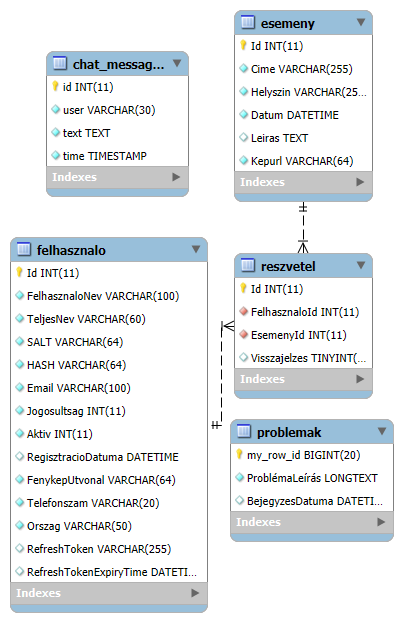
\includegraphics[width=1\textwidth]{tabla.png}
	\end{center}
	\end {figure}
\end{document}